\chapter{Equazioni non lineari del moto e integrazione numerica}

\vspace{-1.5cm} 
\label{sec:equazioni}
In questo capitolo vengono riportate le 12 equazioni differenziali ordinarie (ODE) che costituiscono il modello completo del velivolo, scritte nella forma esplicita pronta per l'integrazione numerica che  avverrà all'interno del capitolo \ref{cap4.6}.

\section{Equazioni di posizione e assetto}
\label{sec:F16AereoFM}
\label{eqAltitudine}
Sviluppando il prodotto matriciale di trasformazione $\mathbf{C}_{tp/frd}$, le derivate della posizione nel Target Plane risultano:
\begin{align}
	\dot{p}_N &= u(c\theta c\psi) + v(s\phi s\theta c\psi - c\phi s\psi) + w(c\phi s\theta c\psi + s\phi s\psi) \\
	\dot{p}_E &= u(c\theta s\psi) + v(s\phi s\theta s\psi + c\phi c\psi) + w(c\phi s\theta s\psi - s\phi c\psi) \\
	\dot{p}_D &= u(-s\theta) + v(s\phi c\theta) + w(c\phi c\theta)
\end{align}
\textbf{Significato Fisico:} La terza equazione $\dot{p}_D$ governa il rateo di discesa. Di conseguenza, il rateo di salita effettivo del velivolo è $\dot{h} = u(s\theta) - v(s\phi c\theta) - w(c\phi c\theta)$.

\subsection*{Equazioni Cinematiche dell'Assetto }
Per aggiornare l'orientamento spaziale del velivolo $\bm{\Phi}$, le velocità angolari di rollio, beccheggio e imbardata misurate in assi FRD vengono proiettate sulle derivate degli angoli di Eulero:
\begin{align}
	\dot{\phi} &= p + q (s\phi \tan\theta) + r (c\phi \tan\theta) \\
	\dot{\theta} &= q (c\phi) - r (s\phi) \\
	\dot{\psi} &= q \left(\frac{s\phi}{c\theta}\right) + r \left(\frac{c\phi}{c\theta}\right)
\end{align}
\textbf{Gimbal Lock:} L'evidente divisione per $c\theta$ nell'equazione di $\dot{\psi}$ dimostra la singolarità matematica a $\theta = \pm 90^\circ$ (volo verticale), risolvibile nell'implementazione software unicamente tramite la cinematica a quaternioni.
\section{Dinamica non lineare delle forze e dei momenti}
Sostituendo $\mathbf{F}_{tot}^{bf} = \mathbf{F}_A^{bf} + \mathbf{F}_T^{bf} + \mathbf{F}_{grav}^{bf}$ e isolando le derivate del vettore velocità $\mathbf{V}_{cm/e}^{frd}$, si ottengono le accelerazioni lineari:
\begin{align}
	\dot{U} &= \frac{X_A + X_T}{m} - g s\theta - (qw - rv) \\
	\dot{V} &= \frac{Y_A + Y_T}{m} + g c\theta s\phi - (ru - pw) \\
	\dot{W} &= \frac{Z_A + Z_T}{m} + g c\theta c\phi - (pv - qu)
\end{align}
\textbf{Significato Fisico:} Le equazioni dimostrano come le forze esterne combinate (aerodinamica $X_A, Y_A, Z_A$ e propulsione $X_T, Y_T, Z_T$) e il vettore gravità continuamente ripartito dagli angoli di assetto, si sommino all'effetto intrinseco di accoppiamento rotazionale (es. $qw - rv$).

\subsection*{Equazioni dei Momenti}
Dal bilancio vettoriale dei momenti $\mathbf{M}^{bf} = [l^{bf}, m^{bf}, n^{bf}]^T$, si estraggono le accelerazioni angolari:
\begin{align}
	l^{bf} &= I_{xx}\dot{p} - I_{xz}\dot{r} + (I_{zz} - I_{yy})qr - I_{xz}pq \\
	m^{bf} &= I_{yy}\dot{q} + (I_{xx} - I_{zz})pr + I_{xz}(p^2 - r^2) \\
	n^{bf} &= I_{zz}\dot{r} - I_{xz}\dot{p} + (I_{yy} - I_{xx})pq + I_{xz}qr
\end{align}



\textbf{Significato Fisico:} Il tensore asimmetrico $I_{xz}$ accoppia matematicamente il rollio $p$ con l'imbardata $r$, mentre i termini non lineari come $qr$ e $pr$ modellano le potenti coppie giroscopiche intrinseche della massa rotante del velivolo.
\subsection*{Equazioni Non-Lineari del Moto Longitudinale}
\label{sec:coeff_aero}
Applicando la proprietà di disaccopiamento mostrate all'interno del libro \texttt{Aircraft Control and Simulation} nello stato di volo livellato, le ODE originarie collassano in un sistema di 5 equazioni differenziali che rappresentano la dinamica del moto longitudinale dell'aereo mostrando come gli ingressi interagiscono con il sistema. In questa formulazione si utilizzano i coefficienti aerodinamici espressi nativamente in assi corpo ($C_X$ e $C_Z$), opportunamente proiettati in assi vento tramite l'angolo d'attacco $\alpha$. Inoltre, si evidenzia esplicitamente la dipendenza dei coefficienti dall'ingresso di controllo dell'elevatore ($\delta_e$) e si include il termine di traslazione del momento $\Delta C_{m_{cg}}$:

{\small
	\begin{align}
		\dot{V}_T &= \frac{1}{m} \Big[ T \cos\alpha + \bar{q} S \big(C_X(\alpha, \delta_e) \cos\alpha + C_Z(\alpha, \delta_e) \sin\alpha\big) \Big] - g \sin(\theta - \alpha) \label{eq:long_vt} \\
		\dot{\alpha} &= q - \frac{1}{m V_T} \Big[ T \sin\alpha + \bar{q} S \big(C_X(\alpha, \delta_e) \sin\alpha - C_Z(\alpha, \delta_e) \cos\alpha\big) \Big] + \frac{g}{V_T} \cos(\theta - \alpha) \label{eq:long_alpha} \\
		\dot{\theta} &= q \label{eq:long_theta} \\
		\dot{q} &= \frac{\bar{q} S \bar{c}}{I_{yy}} \left[ C_m(\alpha, \delta_e) + \frac{\bar{c}}{2 V_T} C_{m_q} q + \Delta C_{m_{cg}} \right] \label{eq:long_q} \\
		\dot{h} &= V_T \sin(\theta - \alpha) \label{eq:long_h}
	\end{align}
}

\textbf{Trasformazione Integrata delle Forze Aerodinamiche:}\\
Si presti particolare attenzione alla formulazione utilizzata nelle equazioni \ref{eq:long_vt} e \ref{eq:long_alpha}. Dal punto di vista della meccanica del volo della galleria del vento, i dati estratti dalle gallerie del vento (database NASA dell'F-16 utilizzatto nei codici matlab) misurano le reazioni vincolari torsiometriche bilanciate in modo solidale alla fusoliera, restituendo perciò coefficienti  aerodinamici in \textit{Assi Corpo} ($C_X, C_Z$). Tuttavia, la sintesi delle leggi di controllo necessita di governare variabili cinematiche espresse in \textit{Assi Vento} ($V_T, \alpha$). 

Per conciliare questi due sistemi di riferimento senza avere errori di interpolazione derivanti da conversioni a priori del database, le equazioni differenziali fungono da "trasformatore di coordinate" in tempo reale. I blocchi trigonometrici racchiusi nelle parentesi tonde operano una proiezione vettoriale :
\begin{itemize}
	\item Il termine $\big(C_X \cos\alpha + C_Z \sin\alpha\big)$ isola la componente delle forze aerodinamiche tangenziale al vettore velocità, e corrisponde rigorosamente all'opposto del coefficiente di Resistenza ($-C_D$).
	\item Il termine $\big(C_X \sin\alpha - C_Z \cos\alpha\big)$ isola la componente perpendicolare al vettore velocità (converso positivo verso il basso), corrispondendo rigorosamente all'opposto del coefficiente di Portanza ($-C_L$).
\end{itemize}
Questa modalità di procedere garantisce che  durante l'integrazione e la linearizzazione numerica ch viene eseguita negli script matlab, il calcolatore legga i dati corretti e li proietta istantaneamente nella direzione del moto, fornendo le derivate di stato esatte da poter utilizzare.
Questo set di ODE regola la dinamica longitudinale e su di esso verrà calcolato il punto di Trim in volo di crociera e tramite linearizzazione si estrarranno le matrici del sistema in spazio di stato ($\mathbf{A}_{long}$, $\mathbf{B}_{long}$, $\mathbf{C}_{long}$, $\mathbf{D}_{long}$). 
\label{cap:5}
È fondamentale notare l'utilizzo di $\mathbf{B}_{ctrl}$ in luogo della matrice di ingresso totale $\mathbf{B}_{long}$: per la sintesi dei controllori, infatti, è strettamente necessario estrarre e separare le sole colonne relative agli ingressi fisicamente comandabili dal computer di volo (attuatori: manetta, elevatore e flap), isolandole dagli ingressi di disturbo non controllabili (come la dinamica delle raffiche di vento, che andranno a formare la matrice separata $\mathbf{B}_{wind}$). La spiegazione completa e l'implementazione analitica di questa scomposizione matriciale è rimandata al \textbf{Capitolo 10} (si veda la Sezione \ref{sec:cap12_1}). \textit{Nota metodologica:} L'implementazione software di questa procedura, che prevede prima la linearizzazione numerica del modello completo a 6-DOF e il successivo filtraggio algoritmico per isolare le sole componenti longitudinali utili alla sintesi dei controllori, verrà trattata in dettaglio nel \textbf{Capitolo 7} (si veda la Sezione \ref{sec:cap8_3}).

\subsection*{Equazione di Uscita: Accelerazione Normale ($a_z$)}
Le variabili di stato $V_T, \alpha, \theta, q$ e $h$ rappresentano gli stati del sistema governati da equazioni differenziali, l'accelerazione misurata dal sensore inerziale lungo l'asse Z del corpo ($a_z$) è una variabile di uscita algebrica e di seguito si mostra il modo in cui si ottiene. 

Come ampiamente discusso in \textit{Aircraft Control and Simulation} (Stevens e Lewis)\cite{stevens2015aircraft}, un accelerometro di bordo non misura l'accelerazione cinematica totale, bensì la \textbf{forza specifica}. Essa rappresenta la risultante delle sole forze esterne non gravitazionali (aerodinamiche e propulsive) agenti sulla massa sismica del sensore, divisa per la massa del velivolo. Matematicamente, lungo l'asse Z del corpo:
\begin{equation}
	a_z = \frac{F_{z,aero} + F_{z,prop}}{m}
\end{equation}

Assumendo che il vettore spinta sia allineato con l'asse longitudinale del velivolo, il segnale $a_z$ deriva interamente dalle forze aerodinamiche.Utilizzando direttamente i coefficienti aerodinamici espressi in assi corpo ($C_X$ e $C_Z$), che costituiscono l'output nativo dei modelli di volo a sei gradi di libertà, la forza aerodinamica normale si esprime banalmente come:
\begin{equation*}
	F_{z,aero} = \bar{q} S C_Z(\alpha, \delta_e)
\end{equation*}

A differenza della formulazione in assi vento (che richiederebbe la complessa scomposizione trigonometrica $F_{z,aero} = -L \cos\alpha - D \sin\alpha$), l'uso degli assi corpo evita ulteriori trasformazioni. Considerando come ingresso di controllo aerodinamico primario esclusivamente l'elevatore ($\delta_e$), l'equazione di uscita definitiva risulta:
\begin{equation}
	a_z = \frac{\bar{q} S}{m} C_Z(\alpha, \delta_e) \label{eq:long_az}
\end{equation}



\textbf{Intervento dell'Elevatore e Matrice $\mathbf{D}_{long}$:}
\textbf{Importanza di $a_z$ nella Teoria dei Controlli:}
L'equazione \ref{eq:long_az} ha un' importanza per la sintesi dei sistemi di controllo di volo, per due ragioni distinte: una di natura matematica e una di natura operativa.

\begin{enumerate}
	\item \textbf{Legame Diretto Ingresso-Uscita (Matrice $\mathbf{D}_{long}$):} 
	Dal punto di vista della modellistica in spazio di stato, poiché il coefficiente di portanza $C_L$ dipende istantaneamente dalla deflessione dell'elevatore $\delta_e$, una variazione del comando produce un salto immediato nel segnale misurato $a_z$, prima ancora che l'assetto del velivolo inizi a variare. Questa relazione crea una \textbf{matrice di trasmissione diretta $\mathbf{D}_{long}$ non nulla}. Fisicamente, questo feed-through modella la dinamica, dove un comando per cabrare genera una temporanea perdita di portanza sulla coda, spingendo inizialmente il baricentro del velivolo verso il basso prima di innescare la salita.
	
	\item \textbf{Gestione del Fattore di Carico:}
	Nel moto longitudinale reale, l'accelerazione $a_z$ è strettamente legata al fattore di carico verticale $n_z$ percepito dal pilota e dalla struttura. L'utilizzo di $a_z$ come variabile di feedback primaria nell'anello di controllo serve a:
	\begin{itemize}
		\item \textbf{Protezione Strutturale e Fisiologica:} Il \textit{Flight Control System} (FCS) dell'F-16 utilizza la lettura continua di $a_z$ per implementare algoritmi di protezione dell'inviluppo di volo (\textit{G-Limiting}). Il controllore "taglia" automaticamente l'autorità dell'elevatore se la manovra rischia di superare i limiti strutturali della cellula (tipicamente $+9g / -3g$), prevenendo cedimenti catastrofici o la perdita di coscienza indotta dall'accelerazione nel pilota (G-LOC).
		\item \textbf{Logica di Comando del Pilota:} Nei moderni caccia \textit{fly-by-wire}, la cloche (side-stick) non comanda fisicamente la deflessione dell'elevatore. Nel volo a medie e alte velocità, la trazione del pilota sulla barra si traduce in una richiesta esplicita di accelerazione (sistema \textit{G-command}). Il controllore regola l'elevatore affinché l'$a_z$ misurata insegua l'$a_z$ comandata dal pilota. Controllare l'accelerazione sull'asse Z significa quindi governare direttamente la curvatura della traiettoria e i "G" percepiti nell'abitacolo, garantendo risposte tattiche prevedibili e letali.
	\end{itemize}
\end{enumerate}.
\section{Meccanismo di Controllo Longitudinale}
Le equazioni \ref{eq:long_vt}-\ref{eq:long_h} e l'equazione \ref{eq:long_az} dimostrano matematicamente come l'ingresso primario dell'elevatore ($\delta_e$) interagisca con l'intera dinamica del velivolo. Nel Capitolo 6 sono mostrati proprio i coefficienti dinamici utilizzati sia per moto longitudinale e latero-direzionale dell'aereo, mostrando come l'ingresso dell'elevatore condiziona i coefficienti aerodinamici al Capitolo (\ref{sec:coefficienti_aerodinamici}):

\begin{enumerate}
	\item \textbf{Azione Primaria su $\dot{q}$ e $a_z$:} 
	La deflessione $\delta_e$ modifica istantaneamente il coefficiente di momento $C_m$ (innescando l'accelerazione angolare $\dot{q}$) e il coefficiente di portanza $C_L$ (misurato istantaneamente dall'accelerometro come variazione di $a_z$).
	\item \textbf{Integrazione su $q$ e $\dot{\theta}$ (Variazione di Assetto):} 
	L'accelerazione $\dot{q}$ si integra nella velocità di beccheggio $q$, la quale forza la rotazione fisica del velivolo variando l'angolo di assetto $\dot{\theta}$ (Equazione \ref{eq:long_theta}).
	\item \textbf{Azione Diretta su $\dot{\alpha}$ (Variazione di Traiettoria):} 
	La variazione di portanza crea l'effetto di \textit{non-minimo fase}: un comando per alzare il muso riduce momentaneamente la portanza totale sulla coda prima che l'angolo $\alpha$ complessivo aumenti.
	\item \textbf{Azione Secondaria su $\dot{V}_T$ (Resistenza Indotta):} 
	Infine, la deflessione meccanica della superficie aggiunge resistenza aerodinamica, alterando $C_D$ e causando una lieve decelerazione iniziale del velivolo.
\end{enumerate}


\section{Rappresentazione dell'assetto mediante quaternioni}
\label{sec:quaternioni}
Come evidenziato dalle equazioni cinematiche dell'assetto, l'uso degli angoli di Eulero ($\bm{\Phi}$) per l'integrazione numerica introduce la singolarità del \textit{Gimbal Lock} a $\theta = \pm 90^\circ$. Inoltre, il motore di rendering (\textit simulatore 3D su flightGear \ref{sec:cinepresa}) all' interno del simulatore affronta un problema correlato ma distinto nell'applicare la rotazione $(\phi, \theta, \psi)$ al modello 3D del velivolo. Se si utilizzassero direttamente le matrici di rotazione di Eulero, si riscontrerebbe il  fenomeno del Gimbal Lock un problema che potrebbe causare gravi \textbf{disturbi visivi} durante la simulazione: il modello 3D "scatterebbe" improvvisamente tra orientamenti diversi, poiché variazioni infinitesime di $\phi$ e $\psi$ produrrebbero variazioni numeriche nella matrice di trasformazione risultante. Per risolvere matematicamente e visivamente questo problema, la formulazione moderna della meccanica del volo \cite{lewis2015ch3}, sostituisce l'integrazione degli angoli di Eulero con l'utilizzo dei \textbf{Quaternioni}  costituiscono una rappresentazione matematica che evita le singolarità degli angoli di Eulero, riducendo il costo computazionale e garantendo una resa grafica priva di artefatti visivi all'interno del simulatore.
\begin{figure}[H]
	\centering
	% Sostituisci il nome del file qui sotto con quello della tua immagine
	\includegraphics[width=0.8\textwidth]{Foto/Gymballock}
	\caption{Rappresentazione visiva del fenomeno del Gimbal Lock: allineamento fisico degli assi di rotazione quando l'angolo di beccheggio raggiunge i $90^\circ$, con conseguente perdita di un grado di libertà.}
	\label{fig:gimbal_lock}
\end{figure}

La trattazione teorica di questa sezione si basa sui concetti esposti nel corso online del MIT.\cite{mit_quaternions}
\paragraph{Definizione matematica del quaternione:} Un quaternione è un numero ipercomplesso a quattro componenti, ideato per rappresentare una rotazione nello spazio tridimensionale Viene definito come:
\begin{equation}
	\mathbf{q} = q_0 + q_1\mathbf{i} + q_2\mathbf{j} + q_3\mathbf{k}
\end{equation}
dove $q_0$ (spesso indicato con $w$) rappresenta la parte scalare e $(q_1, q_2, q_3)$ (corrispondenti a $x, y, z$) la parte vettoriale. Le unità immaginarie obbediscono alle identità fondamentali: $\mathbf{i}^2 = \mathbf{j}^2 = \mathbf{k}^2 = \mathbf{ijk} = -1$.

In notazione vettoriale, scriveremo $\mathbf{q} = [q_0, q_1, q_2, q_3]^T$. Per il Teorema di Rotazione di Eulero, qualsiasi orientamento può essere raggiunto tramite una singola rotazione di un angolo $\theta$ attorno a un asse arbitrario descritto dal versore unitario $\hat{u} = [u_x, u_y, u_z]^T$. Il quaternione esprime questa rotazione come:
\begin{equation}
	\mathbf{q} = \begin{bmatrix} \cos(\theta/2) \\ u_x \sin(\theta/2) \\ u_y \sin(\theta/2) \\ u_z \sin(\theta/2) \end{bmatrix}
\end{equation}
Per rappresentare una rotazione fisica pura, il quaternione deve essere unitario, imponendo il vincolo di norma geometrica:
\begin{equation}
	|\mathbf{q}| = \sqrt{q_0^2 + q_1^2 + q_2^2 + q_3^2} = 1
\end{equation}

\textbf{Topologia Continua e Assenza di Singolarità}\\
La motivazione matematica per cui i quaternioni non soffrono del \textit{Gimbal Lock} risiede nella topologia dello spazio che generano. La rappresentazione a 4 parametri vincolata dalla condizione $|\mathbf{q}| = 1$ definisce una varietà matematica (la 3-sfera $S^3$) che è \textbf{liscia e priva di singolarità}. In questo spazio non esistono punti degeneri. La mappa differenziale dai quaternioni unitari al gruppo delle rotazioni tridimensionali $SO(3)$ è un rivestimento doppio regolare ovunque. Ciò significa che ogni orientamento fisico corrisponde esattamente a due quaternioni antipodali ($\mathbf{q}$ e $-\mathbf{q}$, che applicano la medesima rotazione), ma il passaggio da un assetto all'altro avviene sempre percorrendo un arco continuo sulla superficie di $S^3$, garantendo l'assoluta fluidità visiva nel rendering e la stabilità nell'integrazione differenziale.
\begin{figure}[hbt!]
	\centering
	% Sostituisci il nome del file qui sotto con quello della tua immagine
	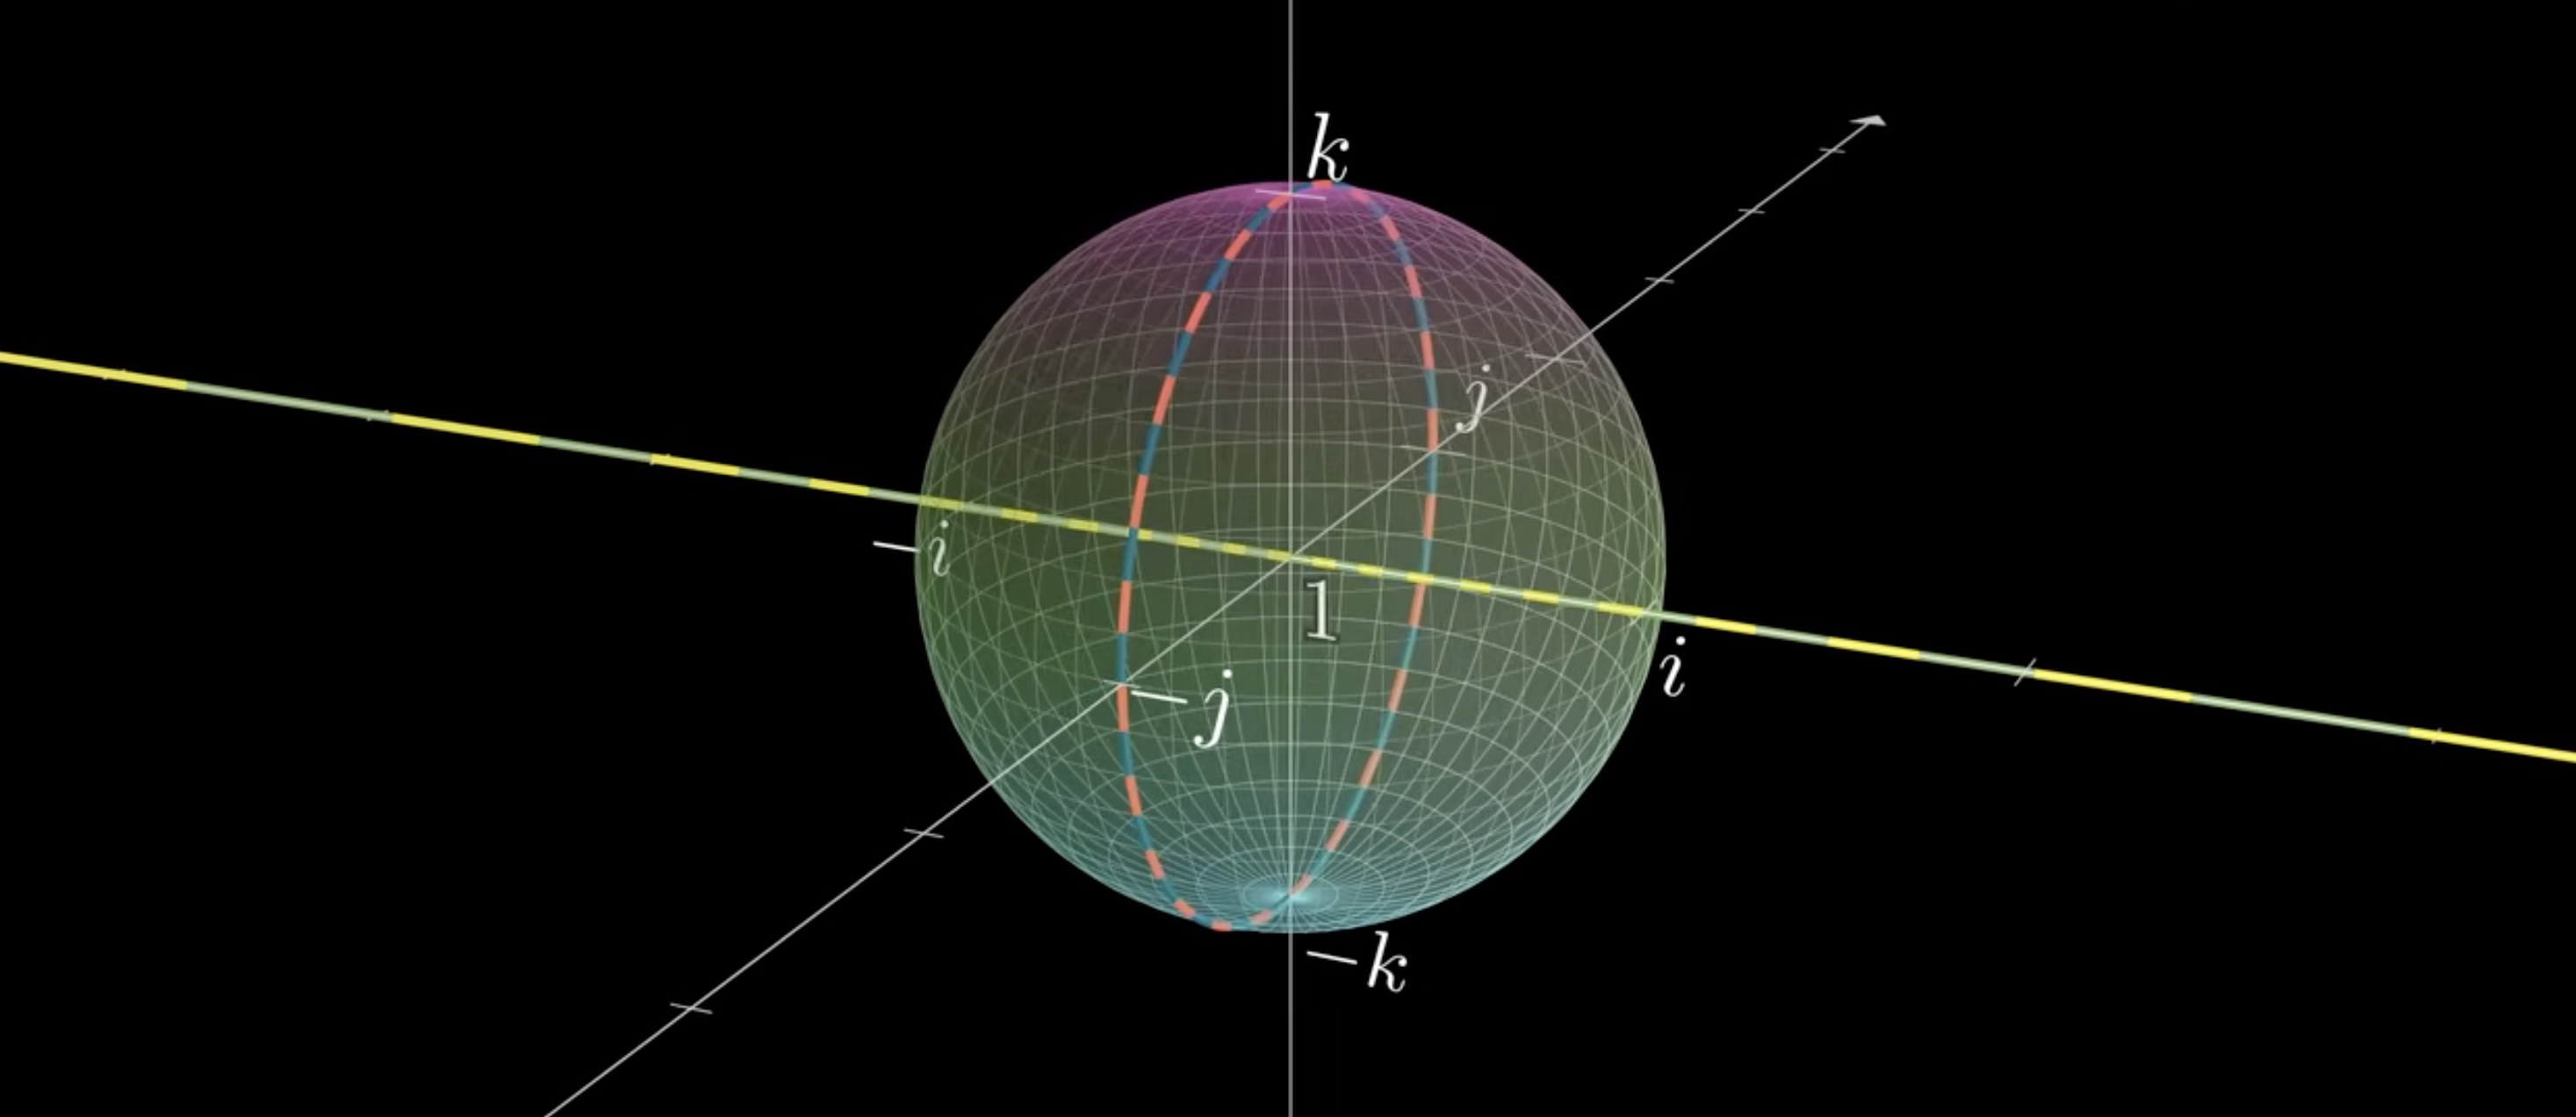
\includegraphics[width=0.99\textwidth]{Foto/quaternionssphere}
	\caption{Rappresentazione topologica della sfera in $S^3$}
	\label{fig:sphere}
\end{figure}

\textbf{Composizione delle Rotazioni}\\
Un ulteriore vantaggio computazionale dei quaternioni rispetto alle matrici dei coseni direttori risiede nella composizione delle rotazioni, che avviene tramite il \textbf{Prodotto di Hamilton} ($\otimes$). Tale operatore, analogamente alle rotazioni fisiche, gode della proprietà associativa ma non di quella commutativa. Dati due quaternioni $\mathbf{p}$ e $\mathbf{q}$, la loro composizione è data da:
\begin{equation}
	\mathbf{p} \otimes \mathbf{q} = 
	\begin{bmatrix}
		p_0 q_0 - p_1 q_1 - p_2 q_2 - p_3 q_3 \\
		p_0 q_1 + p_1 q_0 + p_2 q_3 - p_3 q_2 \\
		p_0 q_2 - p_1 q_3 + p_2 q_0 + p_3 q_1 \\
		p_0 q_3 + p_1 q_2 - p_2 q_1 + p_3 q_0
	\end{bmatrix}
\end{equation}
All'interno dell'architettura di simulazione, le velocità angolari misurate nel Body Frame ($\boldsymbol{\omega}_{b/e}^{frd}$) vengono utilizzate per propagare nel tempo il quaternione tramite una semplice equazione differenziale lineare, ricavando gli angoli di Eulero ($\phi, \theta, \psi$) a posteriori, esclusivamente per l'interfaccia utente o per le leggi di controllo lineari, isolando così il nucleo matematico del simulatore dal rischio di discontinuità numerica.

\section{Analisi critica dei metodi di Eulero}
\label{cap4.6}
I metodi numerici più semplici appartengono alla famiglia di Eulero. Tuttavia, nell'ambito delle simulazioni aerospaziali considerate in questa tesi, tali metodi sono stati esclusi a causa delle loro limitazioni in termini di stabilità e conservazione dell’energia del sistema dinamico, le quali generano un’incertezza tale da rendere inattendibili i risultati ottenuti. \textbf{Eulero in Avanti e Divergenza}\\ Il metodo di Eulero Esplicito calcola lo stato futuro approssimando la curva della soluzione con la sua retta tangente calcolata all'istante iniziale $t_n$:
\begin{equation}
X_{n+1} = X_n + h \cdot f(X_n, U_n, t_n)
\end{equation}
Dal punto di vista geometrico, questo approccio ignora la curvatura della traiettoria di stato all'interno dell'intervallo $h$. Fisicamente, l'errore di troncamento locale, proporzionale a $\mathcal{O}(h^2)$, si traduce in un drammatico effetto di non conservazione dell'energia. Nei sistemi con dinamiche oscillatorie scarsamente smorzate (come il modo Phugoid o il Dutch Roll di un velivolo), Eulero Esplicito agisce come un iniettore artificiale di energia. Ad ogni passo, l'errore di approssimazione tangenziale spinge lo stato leggermente all'esterno dell'orbita reale nello spazio delle fasi. Nel tempo, questa energia spuria si accumula, portando a una divergenza numerica della soluzione, anche se il velivolo reale è fisicamente stabile.

\textbf{Eulero all'Indietro (Implicito) e Smorzamento Numerico}\\
Per ovviare all'instabilità, si potrebbe ricorrere al metodo di Eulero Implicito, che valuta la derivata all'istante futuro:
\begin{equation}
X_{n+1} = X_n + h \cdot f(X_{n+1}, U_{n+1}, t_{n+1})
\end{equation}
Sebbene questo metodo sia incondizionatamente stabile, esso è computazionalmente costoso poiché richiede la risoluzione di un sistema di equazioni non lineari (ad esempio tramite Newton-Raphson) ad ogni step. Peggio ancora, dal punto di vista fisico, Eulero all'Indietro soffre del problema opposto rispetto alla sua variante esplicita: introduce uno smorzamento numerico artificiale. Esso dissipa virtualmente l'energia del sistema, falsando la percezione dei modi dinamici del velivolo, che appariranno più smorzati e stabili di quanto non siano nella realtà aerodinamica.

\section{Metodo di Runge-Kutta del quarto ordine (RK4)}

Per garantire la fedeltà fisica della simulazione rispettando la dinamica reale delle energie in gioco, il testo di Stevens e Lewis\cite{stevens2015aircraft} si affida al metodo di Runge-Kutta del quarto ordine (RK4). Questo metodo esplicito raggiunge un bilanciamento eccellente tra stabilità numerica, accuratezza ed efficienza computazionale. L'errore di troncamento locale è ridotto a $\mathcal{O}(h^5)$, mentre l'errore globale scala come $\mathcal{O}(h^4)$, permettendo di utilizzare passi di integrazione più ampi senza incorrere in divergenze o distorsioni energetiche.

\textbf{Formulazione Matematica}\\
Il metodo RK4 calcola lo stato futuro valutando il campo vettoriale delle derivate $f$ in quattro punti distinti all'interno dell'intervallo temporale $[t_n, t_{n+1}]$, per poi mediarli con pesi specifici derivati dallo sviluppo in serie di Taylor. I quattro incrementi (slopes) vettoriali sono calcolati in sequenza come segue:
\begin{align}
k_1 &= f(X_n, U_n, t_n) \\
k_2 &= f\left(X_n + \frac{h}{2}k_1, U_{n+1/2}, t_n + \frac{h}{2}\right) \\
k_3 &= f\left(X_n + \frac{h}{2}k_2, U_{n+1/2}, t_n + \frac{h}{2}\right) \\
k_4 &= f(X_n + h k_3, U_{n+1}, t_n + h)
\end{align}
Il significato fisico dei quattro predittori è il seguente:
\begin{itemize}
    \item $k_1$ è la pendenza calcolata all'inizio dell'intervallo (equivalente a Eulero in avanti).
    \item $k_2$ è una stima della pendenza al punto medio dell'intervallo, utilizzando $k_1$ per proiettare lo stato.
    \item $k_3$ è una seconda stima (più raffinata) della pendenza al punto medio, utilizzando $k_2$.
    \item $k_4$ è la stima della pendenza alla fine dell'intervallo, utilizzando $k_3$.
\end{itemize}
Infine, lo stato al tempo $t_{n+1}$ viene aggiornato calcolando una media ponderata delle quattro pendenze. I pesi assegnati (1, 2, 2, 1) sono mutuati dalla regola di quadratura di Simpson, che assegna maggior rilevanza alle stime calcolate nel punto medio per massimizzare la fedeltà della traiettoria:
\begin{equation}
X_{n+1} = X_n + \frac{h}{6}(k_1 + 2k_2 + 2k_3 + k_4)
\end{equation}

\textbf{Applicazione al Modello 6-DOF}\\
Nell'architettura del simulatore, ad ogni step temporale, il blocco matematico che implementa le equazioni descritte viene richiamato quattro volte consecutive dal solutore RK4. Ad ogni chiamata, il vettore delle forze aerodinamiche e propulsive viene ricalcolato sulla base degli stati intermedi generati dai coefficienti $k_i$. Questo approccio garantisce che la complessa rete di accoppiamenti non lineari (come le coppie giroscopiche e le dipendenze da $\alpha$ e $\beta$) venga tracciata con una precisione tale da prevenire l'instabilità energetica tipica dei modelli aeronautici complessi ad alti ratei di rotazione.\cite{stevens2015aircraft}
